% ============================================================================
% Relatório do Projeto 1 -- CIC0124 Redes de Computadores (UnB, 2026)
% Formato IEEEtran (conferência), SEM folha de capa, MÁXIMO 8 PÁGINAS (sem anexos).
% Compilar: Overleaf > New Project > Upload Project > relatorio-overleaf.zip > Recompile (pdfLaTeX).
%
% PENDÊNCIAS: tudo em vermelho "[PREENCHER: ...]" (nomes, matrículas, Wireshark, contribuição).
% Todos os números das Seções III-B1 a III-B6 e III-B8 vêm de experimentos/resultados/*.csv
% (execução de 05/11/2026 19:36) e de experimentos/resultados/anteriores/.
% Se passar de 8 páginas: reduza a Fig. 2 (painel) para 0.8\columnwidth ou remova-a.
% ============================================================================
\documentclass[conference]{IEEEtran}

\usepackage[utf8]{inputenc}
\usepackage[T1]{fontenc}
\usepackage[brazilian]{babel}
\usepackage{graphicx}
\usepackage{booktabs}
\usepackage{xcolor}
\usepackage{tikz}
\usetikzlibrary{positioning}
\usepackage{url}

\newcommand{\pend}[1]{\textcolor{red}{[PREENCHER: #1]}}
\newcommand{\figplaceholder}[2]{\fbox{\parbox[c][#2][c]{0.9\columnwidth}{\centering\textcolor{red}{[FIGURA: #1]}}}}
% Capturas do Wireshark: basta enviar figuras/captura1.png (2 e 3) ao Overleaf; enquanto o arquivo
% nao existir, aparece um quadro vermelho no lugar.
\newcommand{\captura}[3]{\IfFileExists{figuras/#1}{\includegraphics[width=\columnwidth]{figuras/#1}}{\figplaceholder{#2 (envie figuras/#1)}{#3}}}

\begin{document}

\title{Projeto 1 --- EcoMonitor: Monitoramento Ambiental em Tempo Real com HTTP e WebSocket e Avaliação Experimental da Comunicação em Rede}

\author{
\IEEEauthorblockN{Vitor Neves Garcia --- Matrícula 252003613}
\IEEEauthorblockA{Departamento de Ciência da Computação, Universidade de Brasília}
}

\maketitle

\begin{abstract}
Apresentamos o EcoMonitor, aplicação distribuída em que sensores simulados enviam medições por HTTP a um servidor que as grava, gera alertas e as publica por WebSocket em painéis Web. Medimos RTT, vazão, concorrência, TCP versus UDP e condições de rede emuladas, e analisamos o tráfego real com o Wireshark.
\end{abstract}

\begin{IEEEkeywords}
HTTP, WebSocket, TCP e UDP, Wireshark
\end{IEEEkeywords}

% ----------------------------------------------------------------------------
\section{Introdução}
Aplicações da Internet combinam clientes Web, servidores, persistência e canais de atualização em tempo real, e seu desempenho depende dos protocolos das camadas de aplicação e de transporte \cite{kurose}. Entender como mensagens são formatadas, encapsuladas, multiplexadas e afetadas por atraso e perda é um objetivo central da disciplina de Redes de Computadores.

Neste trabalho projetamos, implementamos e medimos o \emph{EcoMonitor}, um sistema de monitoramento ambiental com sensores \textbf{simulados} de temperatura, umidade e de um índice de qualidade do ar \textbf{fictício}. O sistema tem cliente Web, servidor acessível pela rede, vários clientes simultâneos identificados de forma independente, HTTP para comandos e consultas, WebSocket para eventos em tempo real, protocolo de aplicação próprio, persistência com histórico, alertas por limiar, autenticação, validação de entradas, logs e ferramentas para medir RTT, vazão e tempo de resposta. As medições foram automatizadas para serem repetíveis, e as condições de atraso, perda e variação foram emuladas por um proxy próprio.

O relatório está organizado assim: a Seção~II apresenta a fundamentação teórica; a Seção~III descreve o cenário, a arquitetura, o protocolo e a metodologia e analisa os experimentos A--E e as capturas no Wireshark; a Seção~IV conclui.

% ----------------------------------------------------------------------------
\section{Fundamentação Teórica}
\textbf{Camadas, encapsulamento e multiplexação.} Cada camada acrescenta seu cabeçalho aos dados da camada superior: a mensagem HTTP vai num segmento TCP, que vai num datagrama IP, que vai num quadro de enlace \cite{kurose}. No destino, o sistema operacional entrega cada segmento ao processo certo pela quádrupla (IP e porta de origem, IP e porta de destino), o que permite que um único processo servidor na porta 8080 atenda muitas conexões simultâneas (multiplexação/demultiplexação).

\textbf{HTTP.} O HTTP é um protocolo de aplicação do tipo requisição/resposta, com métodos, cabeçalhos e códigos de status \cite{rfc9110}. Usamos HTTP/1.1 sobre TCP com conexões persistentes (\emph{keep-alive}): após o primeiro \emph{handshake}, as requisições seguintes reutilizam a mesma conexão.

\textbf{WebSocket.} O WebSocket começa com uma requisição HTTP com \texttt{Upgrade: websocket}; o servidor responde \texttt{101 Switching Protocols} e a mesma conexão TCP passa a transportar quadros nos dois sentidos, sem nova requisição \cite{rfc6455}. É adequado quando o servidor precisa \emph{empurrar} eventos, evitando consultas periódicas (\emph{polling}).

\textbf{TCP e UDP.} O TCP é orientado a conexão (\emph{handshake} de três vias) e entrega um fluxo de bytes confiável e ordenado, com números de sequência, confirmações, retransmissão e controles de fluxo e de congestionamento; no início de uma conexão a janela cresce gradualmente (\emph{slow start}), de modo que transferir muitos dados exige vários RTTs \cite{rfc9293,kurose}. O algoritmo de Nagle pode agrupar mensagens pequenas; a opção \texttt{TCP\_NODELAY} o desliga. O UDP envia datagramas independentes, sem conexão, sem garantia de entrega, de ordem ou de não duplicação \cite{rfc768}: a aplicação precisa detectar e tratar perdas.

\textbf{Protocolo de aplicação e JSON.} Um protocolo de aplicação define formato, campos, sequência de mensagens e tratamento de erros. Usamos JSON \cite{rfc8259} pela legibilidade (inclusive no Wireshark) e pelo suporte nativo no navegador.

\textbf{Métricas.} O \emph{RTT de aplicação} é o tempo entre o envio de uma requisição e o recebimento da resposta completa, medido pelo cliente; ele inclui a rede, as pilhas TCP/IP e o processamento no servidor, que separamos com um cabeçalho de tempo. A \emph{vazão útil} (\emph{goodput}) considera só os bytes da aplicação, sem cabeçalhos. Resumimos amostras por média, mediana, desvio padrão amostral e percentil 95 (p95); a mediana e o p95 são menos sensíveis a valores extremos que a média.

\textbf{Emulação de rede.} Atraso, perda e variação (\emph{jitter}) podem ser impostos no nível de pacote (ex.: Clumsy, no Windows \cite{clumsy}) ou por um \emph{proxy} em espaço de usuário. O \emph{proxy} é simples e não exige privilégios, mas termina a conexão TCP dos dois lados: o kernel nunca vê perda nem o RTT emulado, então perda de segmentos TCP e efeitos de janela não são reproduzidos.

\textbf{Persistência.} O SQLite grava o banco em um arquivo. No modo \emph{Write-Ahead Logging} (WAL), as gravações são anexadas a um log e, com \texttt{synchronous=NORMAL}, o \texttt{fsync} ocorre só nos \emph{checkpoints}, e não a cada transação \cite{sqlite}.

\textbf{Observação.} O Wireshark captura e decodifica quadros de todas as camadas, mostrando encapsulamento, \emph{handshakes}, retransmissões e tempos \cite{wireshark}; no Windows, o tráfego \texttt{127.0.0.1} é capturado pela interface de \emph{loopback} do Npcap.

% ----------------------------------------------------------------------------
\section{Ambiente Experimental e Análise de Resultados}
\subsection{Descrição do Cenário}
\textbf{Hardware e software.} Um computador de mesa ASUS com AMD Ryzen~5 5600 (6 núcleos, 12 \emph{threads}), 16~GiB de RAM e Windows~11 Pro (\emph{build} 26200). Servidor em Java (OpenJDK~27) com Spring Boot 4.1.2 \cite{spring} (Tomcat embutido, Web MVC, WebSocket, JDBC), SQLite \cite{sqlite} via \texttt{sqlite-jdbc}~3.53 e painel em HTML/JavaScript com Chart.js~4.4.7, servido pelo próprio servidor. Sensores, ferramentas de medição e o emulador de rede são programas Java independentes; gráficos em Python/matplotlib. Navegador baseado em Chromium; Wireshark \pend{versão} com Npcap. Código e dados: \pend{URL do repositório}.

\textbf{Topologia.} O servidor escuta em todas as interfaces (\texttt{0.0.0.0:8080}) e aceita clientes de outras máquinas. Nas medições, servidor, clientes e emuladores rodaram na mesma máquina e se comunicaram por \texttt{127.0.0.1} (\emph{loopback}): não há enlace físico nem roteador, o que isola o custo das pilhas e da aplicação; atraso, perda e \emph{jitter} foram emulados (Tabela~\ref{tab:cond}). Usamos \texttt{127.0.0.1} em vez de \texttt{localhost} para evitar ambiguidade IPv4/IPv6 nas medições e nos filtros.

\begin{figure}[t]
\centering
\resizebox{\columnwidth}{!}{%
\begin{tikzpicture}[>=latex, box/.style={draw,rounded corners,align=center,font=\footnotesize,minimum height=0.9cm,inner sep=3pt}]
\node[box] (sens) {Sensores simulados\\(processos Java)};
\node[box,right=1.4cm of sens] (srv) {Servidor Spring Boot\\:8080 (HTTP + WS)};
\node[box,right=1.4cm of srv] (web) {Painéis Web\\(navegadores)};
\node[box,below=0.8cm of srv] (db) {SQLite (WAL)\\\texttt{ecomonitor.db}};
\draw[->] (sens) -- node[above,font=\scriptsize]{HTTP/JSON} node[below,font=\scriptsize]{POST} (srv);
\draw[->] (srv.east) -- node[below,font=\scriptsize]{WebSocket} (web.west);
\draw[->] ([yshift=0.25cm]web.west) -- node[above,font=\scriptsize]{HTTP (GET/PUT)} ([yshift=0.25cm]srv.east);
\draw[<->] (srv) -- node[right,font=\scriptsize]{JDBC} (db);
\end{tikzpicture}}
\caption{Arquitetura centralizada do EcoMonitor e fluxos de comunicação.}
\label{fig:arq}
\end{figure}

\textbf{Arquitetura e escolha dos protocolos.} A arquitetura é centralizada (Fig.~\ref{fig:arq}): o servidor recebe, valida, grava, avalia limites e publica eventos. Usamos HTTP para comandos e consultas, que têm semântica natural de requisição/resposta com códigos de status, e WebSocket para eventos, porque o servidor precisa empurrar medições e alertas sem \emph{polling}. Preferimos WebSocket a \emph{sockets} TCP/UDP diretos porque o navegador não abre \emph{sockets} brutos, e porque o WebSocket já oferece delimitação de mensagens e usa a mesma porta do HTTP. Os sensores usam HTTP (uma requisição por medição): cada envio recebe confirmação ou erro explícito, o que simplifica a validação e o tratamento de falhas.

\textbf{Protocolo de aplicação.} Toda mensagem cliente$\rightarrow$servidor é um objeto JSON com \texttt{versao} (\texttt{1.0}) e \texttt{tipoMensagem} (Tabela~\ref{tab:msgs}). Exemplo de medição enviada por um sensor:
{\footnotesize
\begin{verbatim}
POST /api/medicoes   X-Sensor-Token: <token>
{"versao":"1.0","tipoMensagem":"MEDICAO",
 "sensorId":"SENSOR_001","tipoMedicao":
 "TEMPERATURA","valor":28.5,"unidade":"C",
 "timestamp":"2026-11-04T16:30:00"}
\end{verbatim}
}
\noindent A resposta é \texttt{201} com \texttt{CONFIRMAR\_RECEBIMENTO} ou um \texttt{ERRO} com um de 20 códigos (ex.: \texttt{UNIDADE\_INCOMPATIVEL}, \texttt{VALOR\_FORA\_DA\_FAIXA}, \texttt{TOKEN\_INVALIDO}); mensagem rejeitada não altera o banco e gera aviso no log. Campos, faixas, sequências e exemplos completos estão em \texttt{PROTOCOLO.md}. Um alerta é gerado na \emph{transição} para fora do limite (não a cada medição), e um sensor sem mensagens por 15~s é marcado \texttt{INATIVO}.

\begin{table}[t]
\centering\scriptsize\setlength{\tabcolsep}{4pt}
\caption{Mensagens do protocolo de aplicação EcoMonitor v1.0}
\label{tab:msgs}
\begin{tabular}{@{}lll@{}}
\toprule
Mensagem & Transporte / rota & Autenticação\\
\midrule
\texttt{REGISTRAR\_SENSOR} & POST \texttt{/api/sensores} & chave de registro\\
\texttt{MEDICAO} & POST \texttt{/api/medicoes} & token do sensor\\
\texttt{LOGIN} & POST \texttt{/api/login} & usuário e senha\\
\texttt{CONFIGURAR\_LIMITE} & PUT \texttt{/api/configuracoes} & sessão ADMIN\\
consultas (histórico etc.) & GET \texttt{/api/...} & sessão\\
\texttt{CONFIRMAR\_RECEB.}, \texttt{ERRO} & respostas HTTP & ---\\
\texttt{NOVA\_MEDICAO} & WebSocket \texttt{/ws} & sessão, no\\
\texttt{NOVO\_ALERTA} & (servidor$\rightarrow$painéis) & \emph{handshake}\\
\texttt{SENSOR\_(DES)CONECTADO} & & \\
\bottomrule
\end{tabular}
\end{table}

\begin{figure}[t]
\centering
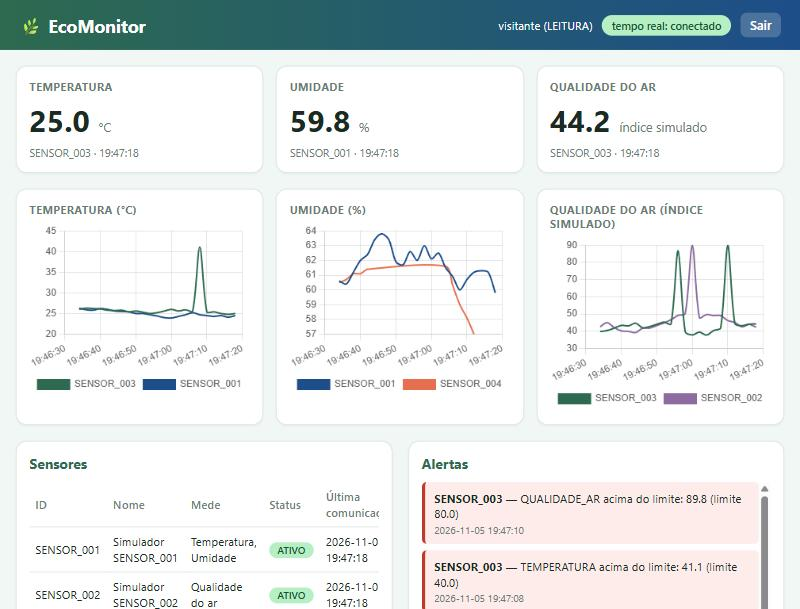
\includegraphics[width=\columnwidth]{figuras/fig_painel.jpg}
\caption{Painel Web do usuário \texttt{visitante} (papel LEITURA) com quatro sensores simulados, atualizado por WebSocket (selo ``tempo real: conectado'').}
\label{fig:painel}
\end{figure}

\textbf{Proteção de dados e pontos de falha.} Senhas são guardadas com PBKDF2-HMAC-SHA256, sal aleatório e 120\,000 iterações; o token de cada sensor é aleatório e guardado como SHA-256; o registro exige uma chave de provisionamento; as consultas, a configuração e o \emph{handshake} WebSocket exigem sessão (ficam abertos só o login, as rotas de apoio aos experimentos e os POSTs dos sensores, autenticados por chave ou token); o papel ADMIN é exigido para alterar limites; todas as entradas são validadas. Limitações: não há TLS, então senhas, tokens e medições trafegam legíveis (confirmado no Wireshark, Seção~III-B7), e a mitigação seria HTTPS/WSS; o token de sessão vai na URL do WebSocket; o servidor é ponto único de falha; as sessões ficam em memória (reiniciar exige novo login); o SQLite admite um escritor por vez.

\textbf{Metodologia de medição.} As medições usam clientes Java (\texttt{HttpClient}, HTTP/1.1, conexão reutilizada) e são disparadas por um único programa (\texttt{RodarExperimentos.java}), que também sobe os servidores de eco e os emuladores. Antes de medir, o servidor é aquecido por 15~s (cerca de 37 mil requisições descartadas) para que o compilador JIT já tenha otimizado o código; em cada série, as 30 primeiras requisições também são descartadas. O servidor devolve no cabeçalho \texttt{X-Tempo-Servidor-Us} o tempo gasto entre a chegada da requisição e o fim da resposta, e a diferença \emph{RTT~$-$~servidor} estima a parcela de rede e pilhas. Painel e simuladores ficaram fechados durante as medições. As condições do Experimento~E (Tabela~\ref{tab:cond}) usam o \texttt{EmuladorRede.java}, um \emph{proxy} TCP/UDP que atrasa cada bloco de dados em cada sentido, sorteia descartes de datagramas UDP e, opcionalmente, aplica atraso uniforme ($\pm$\emph{jitter}), o que pode reordenar datagramas. A condição \texttt{proxy0} passa pelo emulador sem atraso, para isolar o custo do próprio emulador. Fizemos uma execução completa de todas as condições (05/11/2026, 7,2~min) e uma repetição independente da condição \texttt{local}.

\begin{table}[t]
\centering\scriptsize\setlength{\tabcolsep}{4pt}
\caption{Condições de rede (Experimento E), todas em 127.0.0.1}
\label{tab:cond}
\begin{tabular}{@{}lll@{}}
\toprule
Condição & Emulação (por sentido) & Experimentos\\
\midrule
\texttt{local} & nenhuma (linha de base) & A, B, C, D\\
\texttt{proxy0} & \emph{proxy} com atraso 0 & A, D\\
\texttt{atraso50} & 25~ms (RTT $+$50~ms) & A, B, C, D\\
\texttt{perda5} & descarte de 5\% (só UDP) & D\\
\texttt{jitter} & 25~ms $\pm$15~ms, uniforme (só UDP) & D\\
\bottomrule
\end{tabular}
\end{table}

\subsection{Análise de Resultados}
\textbf{1) Validação funcional.} Executamos, com o servidor real: (i) dois painéis simultâneos, \texttt{admin} (ADMIN) e \texttt{visitante} (LEITURA), cada um com sua sessão e sua conexão WebSocket (o log registrou ``total: 2''), ambos recebendo os mesmos eventos (Fig.~\ref{fig:painel}); (ii) quatro sensores simulados simultâneos, com 6 alertas gerados automaticamente em cerca de 1~min (ex.: ``QUALIDADE\_AR acima do limite: 86.7 (limite 80.0)''); (iii) o \texttt{visitante} tentando alterar um limite recebeu \texttt{403 SEM\_PERMISSAO}; (iv) um programa de teste enviou 13 mensagens inválidas (JSON malformado, campo ausente, versão errada, unidade incompatível, valor fora da faixa, tipo não medido pelo sensor, \emph{timestamp} inválido, sem token, token errado, sensor desconhecido, chave de registro errada, \texttt{sensorId} inválido e senha errada) e as 13 receberam o código HTTP e o código de erro esperados, sem gravação no banco; (v) um sensor que silencia por 20~s foi marcado \texttt{INATIVO} e voltou a \texttt{ATIVO} ao retomar o envio, com eventos WebSocket nas duas transições; (vi) com o servidor derrubado, o simulador registrou ``Connection refused'' a cada envio e retomou sozinho quando o servidor voltou; (vii) após reiniciar o servidor, as 172 medições, 6 alertas e 4 sensores gravados continuavam disponíveis no histórico. Todos os eventos aparecem no log com data e hora (console e \texttt{logs/ecomonitor.log}).

\textbf{2) Experimento A --- RTT.} Foram 100 requisições por operação e condição: \texttt{PING} (resposta mínima, sem banco) e \texttt{MEDICAO} (validação, duas gravações no SQLite e publicação WebSocket). A Tabela~\ref{tab:rtt} e a Fig.~\ref{fig:rtt} resumem os resultados.

\begin{table}[t]
\centering\scriptsize\setlength{\tabcolsep}{4pt}
\caption{RTT de aplicação (ms), $n=100$ por linha}
\label{tab:rtt}
\begin{tabular}{@{}llccccc@{}}
\toprule
Condição & Operação & Média & Mediana & DP & p95 & Servidor\textsuperscript{a}\\
\midrule
local & PING & 0,96 & 0,71 & 0,74 & 1,66 & 0,03\\
local & MEDICAO & 1,17 & 0,91 & 1,26 & 1,65 & 0,32\\
proxy0 & PING & 0,93 & 0,83 & 0,30 & 1,37 & 0,04\\
proxy0 & MEDICAO & 1,05 & 0,99 & 0,23 & 1,46 & 0,30\\
atraso50 & PING & 51,06 & 50,98 & 0,32 & 51,60 & 0,05\\
atraso50 & MEDICAO & 51,61 & 51,32 & 2,30 & 52,02 & 0,38\\
\bottomrule
\multicolumn{7}{@{}l}{\scriptsize \textsuperscript{a}Mediana do tempo no servidor (cabeçalho \texttt{X-Tempo-Servidor-Us}).}
\end{tabular}
\end{table}

\begin{figure}[t]
\centering
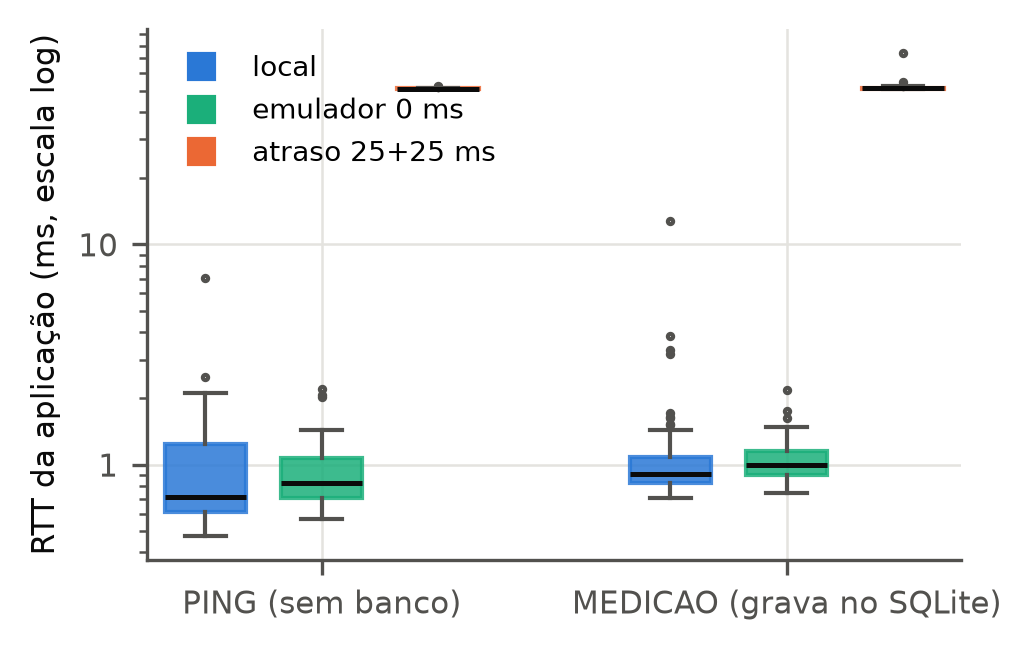
\includegraphics[width=\columnwidth]{figuras/fig_rtt.png}
\caption{Distribuição do RTT de aplicação por operação e condição ($n=100$; caixa: quartis; traço: mediana; pontos: valores extremos). Escala logarítmica.}
\label{fig:rtt}
\end{figure}

Em \emph{loopback}, o RTT mediano fica abaixo de 1~ms. O tempo mediano no servidor sobe de 0,03~ms (PING) para 0,32~ms (MEDICAO), custo da validação, das gravações e da publicação; mesmo assim, a maior parte do RTT local (0,57 a 0,69~ms de mediana) está fora do trecho medido no servidor: pilha HTTP do cliente Java, \emph{parsing} no Tomcat e as pilhas TCP/IP dos dois lados. A média é maior que a mediana por causa de poucos valores extremos (máximo de 12,7~ms na MEDICAO local, quase todo dentro do servidor). O emulador sem atraso acrescenta cerca de 0,1~ms à mediana (0,71$\rightarrow$0,83~ms no PING), desprezível diante dos 50~ms emulados. Com \texttt{atraso50}, o RTT mediano foi 50,98~ms (PING), isto é, o atraso configurado mais $\approx$1~ms, com desvio padrão de só 0,32~ms: o atraso de propagação passa a dominar e o custo do banco vira detalhe.

\textbf{3) Experimento B --- Vazão.} Transferimos corpos de 1~KB a 1~MB em \emph{upload} (POST) e \emph{download} (GET), 10 repetições cada (Fig.~\ref{fig:thr}). Em \texttt{local}, cada transferência de até 100~KB levou menos de 1,2~ms (mediana), então a vazão de mensagens pequenas é limitada pelo custo fixo de cada requisição: cerca de 9 a 10~Mbit/s para 1~KB, contra medianas de 3,4~Gbit/s (\emph{upload}) e 2,8~Gbit/s (\emph{download}) para 1~MB, com grande dispersão (DP de 0,6 a 0,7~Gbit/s). Com \texttt{atraso50}, o tempo ficou em $\approx$51~ms para todos os tamanhos até 100~KB e em 54,2~ms (mediana) para 1~MB, de modo que a vazão cresce quase proporcionalmente ao tamanho (0,16; 1,6; 16 e 155~Mbit/s): uma troca requisição/resposta não supera \emph{tamanho/RTT}. Ressalva: como o \emph{proxy} termina o TCP, o \emph{slow start} não enxerga os 50~ms; numa rede real com esse RTT, transferir 1~MB exigiria vários RTTs, e o emulador \emph{subestima} o tempo das transferências grandes.

\begin{figure}[t]
\centering
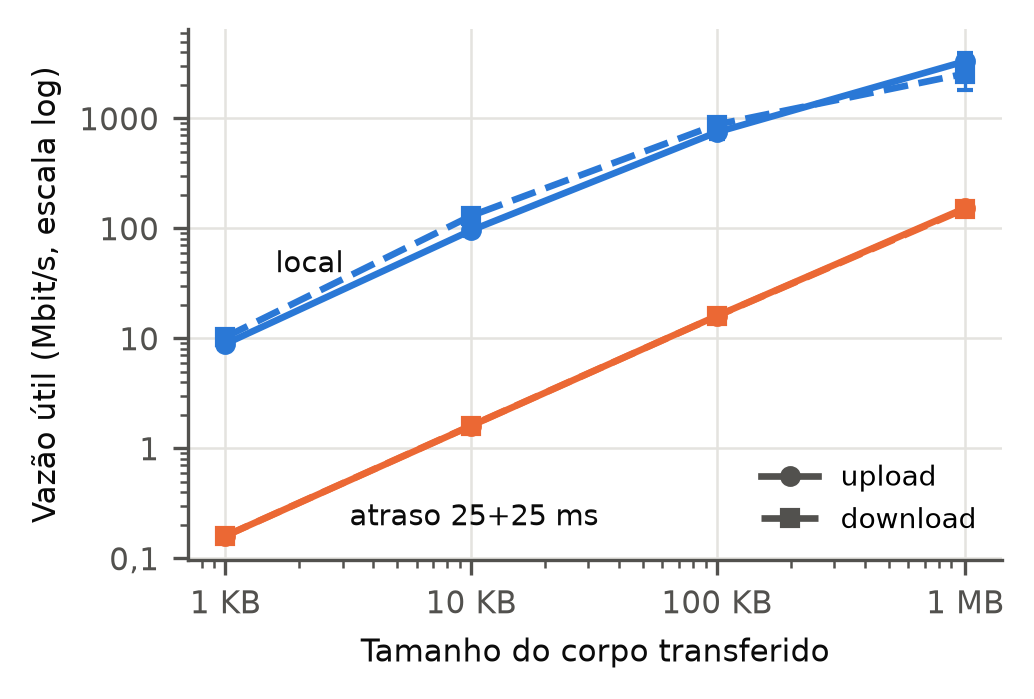
\includegraphics[width=\columnwidth]{figuras/fig_vazao.png}
\caption{Vazão útil (só o corpo) por tamanho, média $\pm$ DP de 10 repetições, condições \texttt{local} e \texttt{atraso50}. Eixos logarítmicos.}
\label{fig:thr}
\end{figure}

\textbf{4) Experimento C --- Concorrência.} Comparamos 1, 2 e 5 clientes simultâneos, cada um com sua conexão TCP e seu sensor, enviando MEDICAO por 30~s com pausa de 100~ms entre envios, e também sem pausa (carga máxima, 15~s) (Tabela~\ref{tab:conc} e Fig.~\ref{fig:conc}). Nenhuma das 76\,346 requisições falhou.

\begin{table}[t]
\centering\scriptsize\setlength{\tabcolsep}{4pt}
\caption{Concorrência: taxa agregada (msg/s) e latência da MEDICAO (ms)}
\label{tab:conc}
\begin{tabular}{@{}lcrccr@{}}
\toprule
Condição & Clientes & Taxa & Mediana & p95 & Máx.\\
\midrule
local, 100~ms & 1 & 9,2 & 1,75 & 2,54 & 13,7\\
 & 2 & 18,4 & 1,66 & 2,74 & 15,1\\
 & 5 & 45,8 & 1,39 & 2,88 & 25,0\\
\midrule
local, sem pausa & 1 & 1685 & 0,38 & 0,64 & 1085\\
 & 2 & 1546 & 0,47 & 0,81 & 540\\
 & 5 & 1601 & 1,13 & 1,80 & 275\\
\midrule
atraso50, 100~ms & 1 & 6,3 & 51,72 & 52,40 & 61,2\\
 & 2 & 12,7 & 51,89 & 52,65 & 71,0\\
 & 5 & 31,7 & 51,73 & 52,71 & 76,4\\
\bottomrule
\end{tabular}
\end{table}

\begin{figure}[t]
\centering
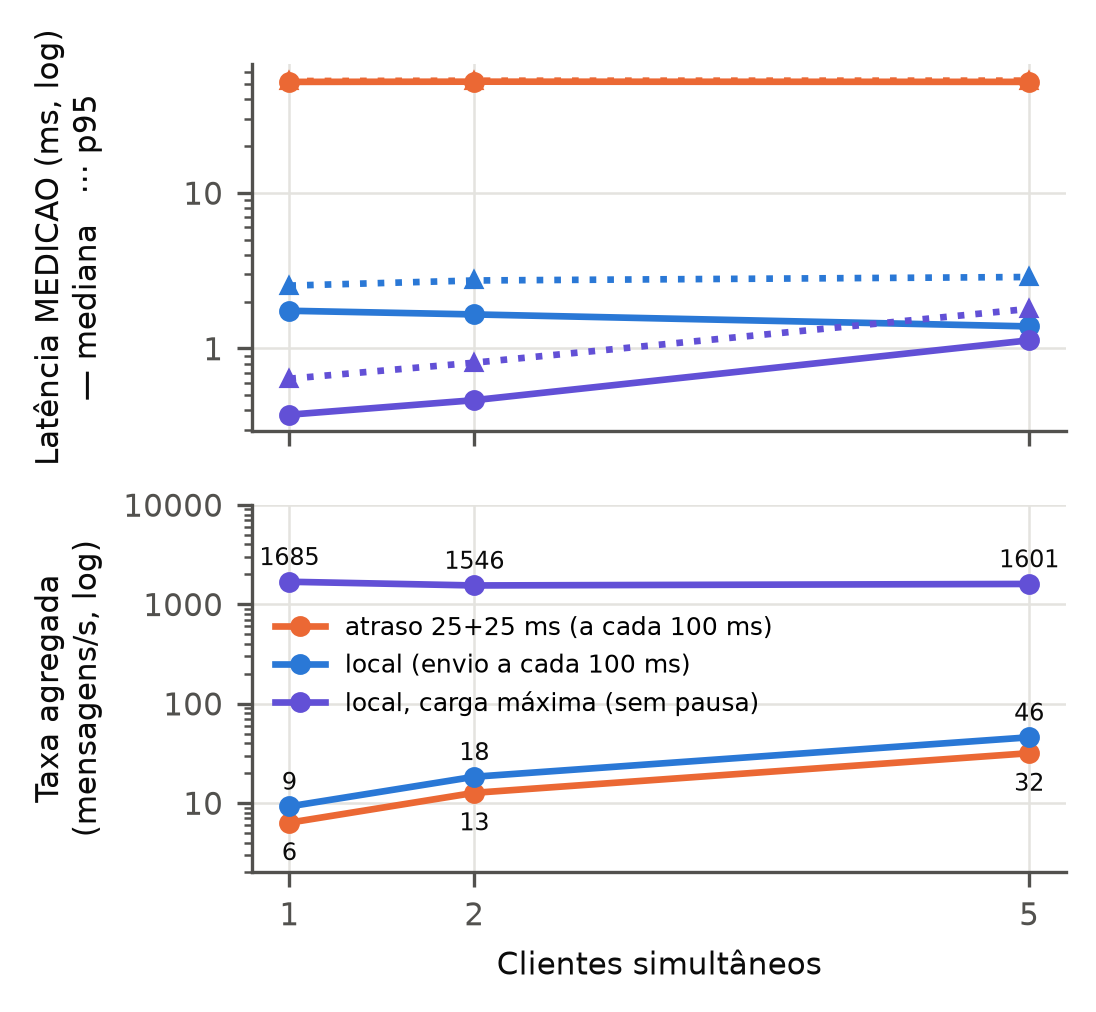
\includegraphics[width=\columnwidth]{figuras/fig_concorrencia.png}
\caption{Latência da MEDICAO (mediana e p95) e taxa agregada em função do número de clientes simultâneos. Escalas logarítmicas.}
\label{fig:conc}
\end{figure}

Com pausa de 100~ms, a taxa cresce linearmente com o número de clientes (9,2$\rightarrow$18,4$\rightarrow$45,8~msg/s) e a latência mediana não piora: o servidor não está saturado. Sem pausa, a taxa agregada \emph{não} cresce com mais clientes (cerca de 1,5 a 1,7 mil msg/s) e a latência mediana triplica de 1 para 5 clientes (0,38$\rightarrow$1,13~ms), sinal de fila em um recurso serializado. Um candidato é o \emph{pool} de uma única conexão SQLite, pela qual passam as quatro operações SQL de cada MEDICAO; como cliente e servidor dividem a mesma CPU, não isolamos a causa. Na repetição independente, a taxa sem pausa variou mais (749, 1713 e 1292~msg/s para 1, 2 e 5 clientes), mas a tendência da latência se repetiu (0,43; 0,47; 1,12~ms): a diferença de taxa entre 1, 2 e 5 clientes nessa faixa não é significativa, a ausência de ganho de escala sim. Os máximos de até 1,1~s são raros (o p95 ficou abaixo de 2~ms) e não investigamos sua causa (candidatos: \emph{checkpoints} do WAL ou coleta de lixo). Com \texttt{atraso50}, a latência fica constante em $\approx$51,8~ms e cada cliente envia no máximo $1/(0{,}1+0{,}052)\approx6{,}6$~msg/s, pois espera a resposta antes do envio seguinte: a taxa medida (6,3~msg/s por cliente) passa a ser limitada pelo RTT, não pelo servidor.

\textbf{5) Experimento D --- TCP versus UDP.} Um microteste de eco envia 1000 mensagens numeradas de 100~B a cada 10~ms, com a mesma carga para TCP (com \texttt{TCP\_NODELAY}) e UDP; o cliente mede RTT de aplicação, perdas, duplicatas e mensagens fora de ordem pela sequência (Tabela~\ref{tab:tcpudp}, Fig.~\ref{fig:tcpudp}).

\begin{table}[t]
\centering\scriptsize\setlength{\tabcolsep}{4pt}
\caption{Eco TCP e UDP com carga idêntica (1000 mensagens de 100~B a cada 10~ms); RTT em ms}
\label{tab:tcpudp}
\begin{tabular}{@{}llcccc@{}}
\toprule
Condição & Proto. & Perdidas & Fora de ordem & RTT mediano & RTT p95\\
\midrule
local & TCP & 0 & 0 & 0,061 & 0,099\\
local & UDP & 0 & 0 & 0,094 & 0,152\\
proxy0 & TCP & 0 & 0 & 0,141 & 0,226\\
proxy0 & UDP & 0 & 0 & 0,188 & 0,330\\
atraso50 & TCP & 0 & 0 & 50,11 & 50,19\\
atraso50 & UDP & 0 & 0 & 50,18 & 50,32\\
perda5 & UDP & 86 (8,6\%) & 0 & 0,176 & 0,269\\
jitter & UDP & 0 & 222 & 50,56 & 71,03\\
\bottomrule
\end{tabular}
\end{table}

\begin{figure}[t]
\centering
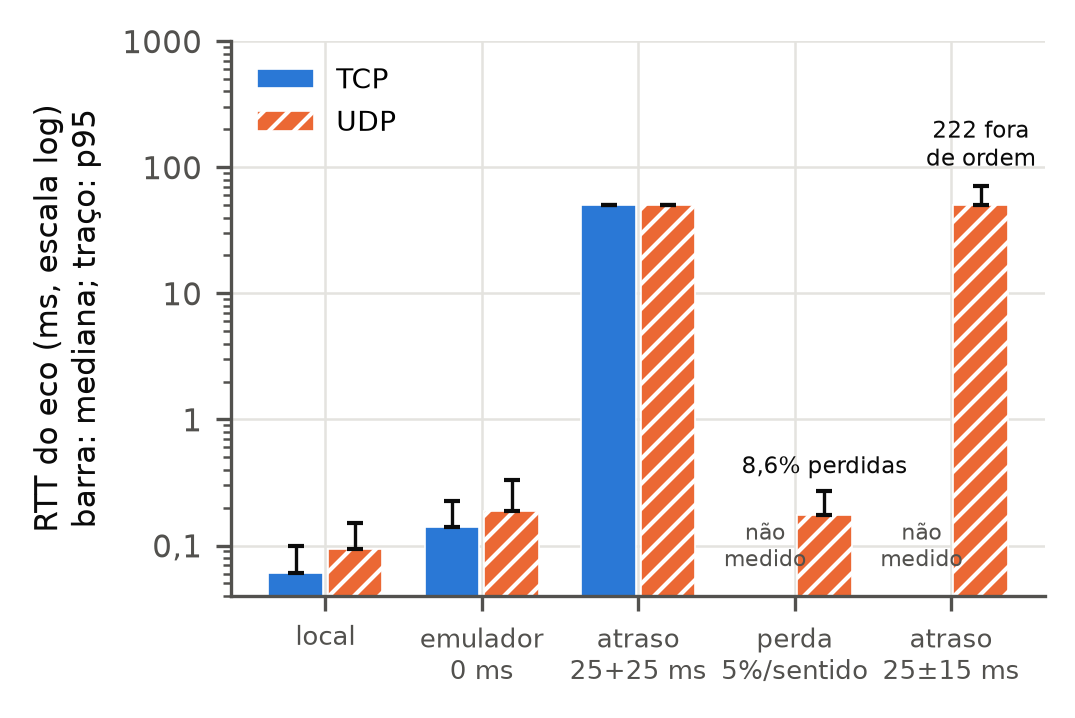
\includegraphics[width=\columnwidth]{figuras/fig_transporte.png}
\caption{RTT do eco TCP e UDP por condição (barra: mediana; traço: p95), com perdas e reordenação anotadas. TCP não foi medido nas condições de perda e \emph{jitter} (ver texto).}
\label{fig:tcpudp}
\end{figure}

Em \emph{loopback} e com atraso fixo, nenhum dos dois perdeu ou reordenou mensagens, e os RTTs ficaram na casa de dezenas de microssegundos; a diferença de $\approx$0,03~ms a favor do TCP reflete as implementações de \emph{sockets} do Java e do Windows usadas no teste, não uma propriedade dos protocolos, e não deve ser generalizada. Com descarte de 5\% por sentido, o UDP perdeu 86 de 1000 mensagens (8,6\%); o esperado é $1-0{,}95^2=9{,}75\%$, com desvio binomial de 0,94 ponto percentual, e o emulador registrou 45 descartes na ida e 41 na volta, coerente com o cliente. O UDP não avisa a aplicação: as perdas só foram detectadas porque o protocolo de teste numera as mensagens. Com \emph{jitter}, 222 mensagens (22,2\%) chegaram fora de ordem, e o RTT variou entre 21,9 e 79,8~ms (limites teóricos: 20 e 80~ms) com DP de 12,3~ms, praticamente o valor teórico da soma de duas uniformes de largura 30~ms ($\sqrt{2\cdot30^2/12}\approx12{,}2$~ms), o que valida o emulador. Sob as mesmas condições, o TCP entregaria tudo e em ordem, retransmitindo e segurando dados no receptor à custa de latência; como o \emph{proxy} não provoca perda de segmentos TCP, essa comparação exigiria emulação no nível de pacote (Clumsy). Os dois protocolos não são funcionalmente equivalentes: o TCP oferece confiabilidade e ordem; o UDP deixa essas tarefas para a aplicação.

\textbf{6) Experimento E --- Condições de rede.} A Tabela~\ref{tab:cond} resume as condições. Os resultados das Seções III-B2 a III-B5 mostram que (i) o atraso emulado soma-se ao RTT de forma quase exata (+50~ms configurados, +50,3~ms medidos na mediana do PING) e passa a dominar todas as métricas; (ii) a vazão de transações requisição/resposta fica limitada por \emph{tamanho/RTT}; (iii) na concorrência, o atraso reduz em 31\% a taxa por cliente (9,2$\rightarrow$6,3~msg/s) sem alterar a latência com mais clientes, pois o gargalo passa a ser a espera pela rede; e (iv) perda e \emph{jitter} expõem diretamente a aplicação UDP. Limitações: emulação em espaço de usuário, sem perda de segmentos TCP nem efeitos de janela; tudo em uma única máquina.

\textbf{7) Análise com Wireshark.} As capturas foram feitas na interface \emph{Adapter for loopback traffic capture} do Npcap, com o cenário de cada uma montado por um script (\texttt{CAPTURA-1.bat} a \texttt{CAPTURA-3.bat}); os arquivos \texttt{.pcapng} estão no repositório (\texttt{experimentos/capturas/}).

\begin{figure}[t]
\centering
\captura{captura1.png}{Captura 1: SYN, SYN-ACK, ACK e POST /api/medicoes com resposta 201}{2.4cm}
\caption{Captura 1 (\pend{data e hora}): \emph{handshake} TCP e requisição/resposta HTTP de um sensor. Filtro: \texttt{tcp.port == 8080}.}
\label{fig:cap1}
\end{figure}

\emph{Captura 1 --- HTTP e TCP} (Fig.~\ref{fig:cap1}; cenário: um sensor envia 6 medições, uma a cada 2~s, seguidas de 5 PINGs; painel fechado). O \emph{handshake} SYN, SYN-ACK, ACK ocorre entre \texttt{127.0.0.1:}\pend{porta de origem} e \texttt{127.0.0.1:8080}, seguido de \texttt{POST /api/sensores} e dos \texttt{POST /api/medicoes} na \emph{mesma} conexão (mesmo \texttt{tcp.stream}), o que confirma o \emph{keep-alive}. O encapsulamento visível é \emph{Null/Loopback} $\rightarrow$ IPv4 $\rightarrow$ TCP $\rightarrow$ HTTP $\rightarrow$ JSON: no \emph{loopback} não há Ethernet, e cada quadro carrega 4~B do cabeçalho de \emph{loopback}, 20~B do IPv4 e o cabeçalho TCP (20~B sem opções). O corpo JSON de uma medição tem \pend{Content-Length} bytes, e o quadro que o transporta tem \pend{Length} bytes. O JSON, o \texttt{X-Sensor-Token} e o cabeçalho \texttt{X-Tempo-Servidor-Us} aparecem em texto puro: sem TLS, qualquer observador da rede os lê.

\begin{figure}[t]
\centering
\captura{captura2.png}{Captura 2: 101 Switching Protocols, quadros WebSocket e Conversations (TCP)}{2.4cm}
\caption{Captura 2 (\pend{data e hora}): resposta \texttt{101 Switching Protocols} e quadros WebSocket empurrados pelo servidor. Filtro: \texttt{http.response.code == 101 || websocket}.}
\label{fig:cap2}
\end{figure}

\emph{Captura 2 --- WebSocket e multiplexação} (Fig.~\ref{fig:cap2}; cenário: dois painéis e três sensores por 30~s). A requisição \texttt{GET /ws?token=...} com \texttt{Upgrade: websocket} recebe \texttt{101 Switching Protocols}; depois, quadros de texto do servidor para o navegador carregam \texttt{NOVA\_MEDICAO} sem nenhuma requisição do navegador, isto é, o servidor empurra os dados. Em \emph{Statistics > Conversations > TCP} (limitado a \texttt{tcp.port == 8080}) aparecem \pend{n} conexões distintas \texttt{127.0.0.1:}\emph{porta efêmera} $\leftrightarrow$ \texttt{127.0.0.1:8080}, uma por sensor e uma ou mais por painel (página e WebSocket): um único processo na porta 8080 as distingue pela quádrupla, o que evidencia a multiplexação. A comunicação é fim a fim entre os processos; numa rede real haveria roteadores e, possivelmente, NAT no caminho.

\begin{figure}[t]
\centering
\captura{captura3.png}{Captura 3: Conversations (UDP) nos dois trechos do emulador}{2.4cm}
\caption{Captura 3 (\pend{data e hora}): perdas UDP inferidas pela contagem de datagramas nos dois trechos do emulador. Filtro: \texttt{udp.port == 9203 || udp.port == 9090}.}
\label{fig:cap3}
\end{figure}

\emph{Captura 3 --- perdas UDP} (Fig.~\ref{fig:cap3}; cenário: eco UDP através do emulador com 5\% de descarte por sentido). Como o emulador é um processo intermediário, a captura vê os quatro trechos: cliente$\rightarrow$emulador (\pend{n}), emulador$\rightarrow$eco (\pend{n}), eco$\rightarrow$emulador (\pend{n}) e emulador$\rightarrow$cliente (\pend{n}). A diferença entre trechos consecutivos é a perda em cada sentido, sem retransmissão, e confere com o \texttt{perdidos} do cliente (Tabela~\ref{tab:corr}).

\begin{table}[t]
\centering\scriptsize\setlength{\tabcolsep}{4pt}
\caption{Correlação entre medições da aplicação e do Wireshark}
\label{tab:corr}
\begin{tabular}{@{}lcc@{}}
\toprule
Medida & Aplicação & Wireshark\\
\midrule
MEDICAO, as 6 da Captura 1, mediana (ms) & \pend{ms} & \pend{ms}\\
PING, Captura 1 (Wireshark) e Exp.~A (ms) & 0,71 & \pend{ms}\\
Perda UDP na Captura 3 (mensagens) & \pend{n} & \pend{n}\\
\bottomrule
\multicolumn{3}{@{}l}{\scriptsize Wireshark: campo \texttt{http.time} (\emph{Time since request}) das respostas.}
\end{tabular}
\end{table}

Para as mesmas seis medições da Captura 1, a mediana do \texttt{http.time} foi \pend{ms}~ms e a do RTT impresso pelo sensor, \pend{ms}~ms. O Wireshark mede do envio da requisição à chegada da resposta na interface, sem a pilha HTTP do cliente Java, por isso seu valor é menor; a diferença é o custo do cliente. \pend{confira e mantenha só se for verdade: os dois valores são maiores que os 0,91~ms do Experimento~A porque, na captura, o servidor não foi aquecido e as requisições são espaçadas de 2~s}. Na Captura~3, as perdas inferidas pelas contagens do Wireshark coincidem com as contadas pelo cliente.

\textbf{8) Problemas e ajustes.} (i) \emph{Banco}: na primeira execução, com o modo de \emph{journal} padrão do SQLite (um \texttt{fsync} a cada gravação), a MEDICAO levava 15,5~ms em média (14,8~ms dentro do servidor), a concorrência com 1 cliente teve média de 362~ms com picos de 0,8~s, e a carga máxima não passou de 49~msg/s. Com WAL e \texttt{synchronous=NORMAL}, a MEDICAO caiu para 0,91~ms (mediana) e a carga máxima subiu para $\approx$1,6 mil msg/s; o custo é que uma queda de energia pode perder as últimas transações, sem corromper o banco \cite{sqlite}. (ii) \emph{Aquecimento}: sem aquecer o servidor, a primeira condição medida pegava o JIT frio (tempo no servidor da MEDICAO de 1,28~ms contra 0,26~ms depois), o que invertia a comparação \texttt{local}~$\times$~\texttt{proxy0}; adicionamos os 15~s de aquecimento. (iii) \emph{Timer do Windows}: com a resolução padrão de 15,6~ms, o emulador configurado para 50~ms produziu 63,7~ms ($\approx$2$\times$31,25~ms); passamos a dormir até 20~ms antes do instante e completar a espera ativamente, o que deu 51,1~ms. (iv) \emph{Perda TCP}: o \emph{proxy} não descarta segmentos TCP; essa medição fica para o Clumsy. As execuções descartadas estão arquivadas no repositório.

% ----------------------------------------------------------------------------
\section{Conclusões}
O EcoMonitor atende aos requisitos do projeto: HTTP para comandos e consultas, WebSocket para eventos empurrados pelo servidor, protocolo JSON próprio com 20 códigos de erro, persistência, alertas, autenticação e tratamento de falhas, validados com dois painéis e quatro sensores simultâneos. Em \emph{loopback}, o RTT mediano ficou abaixo de 1~ms e foi dominado pelas pilhas dos processos, não pelo banco, depois de trocar o \emph{journal} do SQLite por WAL (de 15,5 para 0,91~ms). Sem pausa, a taxa agregada não cresceu com mais clientes ($\approx$1,5 a 1,7 mil msg/s). Com 50~ms emulados, o atraso dominou RTT, vazão e taxa por cliente. TCP e UDP se igualaram sem perturbações, mas, sob perda e \emph{jitter}, o UDP perdeu 8,6\% e reordenou 22\% das mensagens, sem aviso à aplicação. O Wireshark confirmou o \emph{handshake}, o \emph{keep-alive}, o WebSocket e a ausência de TLS. Trabalhos futuros: HTTPS/WSS, banco cliente-servidor, emulação no nível de pacote e testes entre máquinas distintas.

% ----------------------------------------------------------------------------
\begin{thebibliography}{10}
\bibitem{kurose} J.~F. Kurose and K.~W. Ross, \emph{Redes de Computadores e a Internet: Uma Abordagem Top-Down}, 8.~ed. São Paulo: Pearson, 2021.
\bibitem{rfc9110} R.~Fielding, M.~Nottingham, and J.~Reschke, ``HTTP Semantics,'' RFC 9110, IETF, 2022.
\bibitem{rfc6455} I.~Fette and A.~Melnikov, ``The WebSocket Protocol,'' RFC 6455, IETF, 2011.
\bibitem{rfc9293} W.~Eddy, ``Transmission Control Protocol (TCP),'' RFC 9293, IETF, 2022.
\bibitem{rfc768} J.~Postel, ``User Datagram Protocol,'' RFC 768, IETF, 1980.
\bibitem{rfc8259} T.~Bray, ``The JavaScript Object Notation (JSON) Data Interchange Format,'' RFC 8259, IETF, 2017.
\bibitem{wireshark} Wireshark Foundation, ``Wireshark User's Guide.'' [Online]. Disponível: \url{https://www.wireshark.org/docs/}
\bibitem{spring} Broadcom, ``Spring Boot Reference Documentation.'' [Online]. Disponível: \url{https://docs.spring.io/spring-boot/}
\bibitem{sqlite} SQLite Consortium, ``Write-Ahead Logging.'' [Online]. Disponível: \url{https://www.sqlite.org/wal.html}
\bibitem{clumsy} J.~Gao, ``clumsy: makes your network condition on Windows significantly worse.'' [Online]. Disponível: \url{https://github.com/jagt/clumsy}
\end{thebibliography}

% ----------------------------------------------------------------------------
% ANEXOS (não contam nas 8 páginas)
\appendices
\section{Contribuição individual}
\begin{table}[h]
\centering\scriptsize\setlength{\tabcolsep}{4pt}
\begin{tabular}{@{}lll@{}}
\toprule
Autor (matrícula) & Atividades & Participação\\
\midrule
Vitor Neves Garcia (252003613) & todas (trabalho individual) & 100\%\\
\bottomrule
\end{tabular}
\end{table}
\noindent Projeto realizado individualmente: arquitetura, servidor, protocolo, painel, simuladores, experimentos, capturas, relatório e vídeo.

\section{Ferramentas, bibliotecas e uso de IA}
Bibliotecas: Spring Boot 4.1.2 (Web MVC, WebSocket, JDBC), \texttt{org.xerial:sqlite-jdbc}, Chart.js 4.4.7 e matplotlib. Ferramentas: OpenJDK, Maven (\emph{wrapper}), IntelliJ IDEA, Python, Wireshark/Npcap. O código-fonte, as ferramentas de medição e o texto deste relatório foram elaborados com apoio do assistente de IA Claude (Anthropic); o autor revisou, testou e executou o sistema. Todos os números vêm de execuções reais dos programas do repositório (\texttt{experimentos/resultados/}).

\section{Reprodução}
Na raiz do repositório (Windows, JDK~17+): \texttt{1-SERVIDOR.bat} sobe o servidor; \texttt{6-EXPERIMENTOS.bat} roda os Experimentos A--E e gera os gráficos; \texttt{DEMO.bat} sobe servidor, três sensores e o painel. Detalhes no \texttt{README.md} e em \texttt{experimentos/ROTEIRO-EXPERIMENTOS.md}.

\end{document}
